\documentclass{article}
\usepackage[utf8]{inputenc}
\usepackage{amsmath}
\usepackage{graphicx}
\usepackage[a4paper, total={6in, 10in}]{geometry}
\usepackage{float}
\usepackage{caption}
\usepackage{hyperref}
\usepackage{subcaption}
\newcommand{\xdashrightarrow}[2][]{\ext@arrow 0359\rightarrowfill@@{#1}{#2}}
\usepackage{comment}

\title{Big data 2}
\author{Anton Rosenberg}
\date{May 2022}

\begin{document}

\maketitle
\newpage
\section{a}
\subsection{Results}
During this task noise was added to a random set of pictures and then the accuracy of three different classifiers (SVM 'rbf' kernel, Logistic regression with l2 penalisation and 'lbfgs' solver, Random forest) were measured. The score was calculated in the same way as in 1 a where the classifiers hyper parameters were fitted using cross validation on training set and then the three models were fitted on training data and the score was taken on the test data. No prepossessing was made except for normalisation so that all pixels take values between 0 and 1. Since the method was exactly the same for this exercise as in 1 a we can compare these results in order to see how the noise affects the different classifiers. The noise added had two different levels 100 and 255 were a value of 100 means that every pixel in the noisy picture is modified with a value between 0 and 100/255 see figure \ref{noise pics} for an example, the value which every pixel was modified with was drawn from a uniform distribution. The results from the simulations are shown in tables \ref{SVM table}, \ref{RF table} and \ref{LR table}. Looking at the score for the SVM we can see that the noise has an negative impact on the accuracy of the model were it's affected by both the noise level and the number of noisy pictures. However the performance is still a lot better than 50 \% so the model learns something even when half the pictures are noisy. However the performance of the SVM model is worsened by almost 25 \%. For the Logistic Regression model we can see that the noise doesn't appear to have an big effect on the performance of the model were maximum noise and number of noisy pictures only worsens performance by about 8.6 \%. The Random Forest model seem to be the least affected by lower noise levels, and even an higher score was achieved for low noise than the base case without noise in 1a. However the performance worsened by at most 11 \% which is more than the Logistic Regression for higher noise. As for how many of the miss classified pictures the noisy make up they are only slightly over represented. They could however affect the models even if they are not miss classified in the training since they could lead to the model over fitting on the noise.        
\subsection{Conclusions}
We can conclude that the SVM model is most susceptible to noise out of the three classifiers used, this is likely an effect of the low bias kernel used, the noise resistivity of the SVM could be increased by using a higher bias kernel like for example a linear one. Moreover the Logistic Regression and Random Forest classifiers seem to be less affected by noise. The random forest classifier could be good against noise since a noisy picture only affects one decision tree therefore when we add decision trees the tendency for the model to overfit to the noise goes down. 
\begin{table}[H]
    \centering
    \begin{tabular}{c|c|c|c|c|c|c|c}
   Model: SVM \\
    Noise level  & 100 & 100 & 100 & 255 & 255 & 255 \\
       Number noisy pics & 10 & 40 & 100 & 10& 40 & 100 \\
        Percentage noise in errors & 0.08& 0.1 & 0.67 & 0.12& 0.38& 0.67  \\
       Accuracy & 0.76 & 0.74 & 0.66 & 0.67 & 0.68 & 0.65 \\
       Std & 0.03& 0.04 & 0.05 & 0.03 & 0.05 & 0.05\\
    \end{tabular}
    \caption{Caption}
    \label{SVM table}
\end{table}
\begin{table}[H]
\centering
    \begin{tabular}{c|c|c|c|c|c|c|c}
   Model: Logistic Regression \\
    Noise level  & 100 & 100 & 100 & 255 & 255 & 255 \\
       Number noisy pics & 10 & 40 & 100 & 10& 40 & 100 \\
        Percentage noise in errors & 0.13& 0.15 & 0.51 & 0.12 & 0.45& 0.62  \\
       Accuracy & 0.75 & 0.77 & 0.74 & 0.76 & 0.73 & 0.7 \\
       Std & 0.04& 0.05 & 0.06 & 0.05 & 0.05 & 0.05\\
    \end{tabular}
    \caption{Caption}
    \label{LR table}
\end{table}
\begin{table}[H]
\centering
    \begin{tabular}{c|c|c|c|c|c|c|c}
   Model: Random Forest \\
    Noise level  & 100 & 100 & 100 & 255 & 255 & 255 \\
       Number noisy pics & 10 & 40 & 100 & 10& 40 & 100 \\
        Percentage noise in errors & 0.04& 0.23 & 0.4 & 0.03 & 0.13& 0.45\\
       Accuracy & 0.79 & 0.8 & 0.77 & 0.77 & 0.74 & 0.7 \\
       Std & 0.03& 0.03 & 0.04 & 0.06 & 0.04 & 0.05\\
    \end{tabular}
    \caption{Caption}
    \label{RF table}
\end{table}
\begin{figure}[H]
\begin{subfigure}{.5\textwidth}
  \centering
  % include first image
  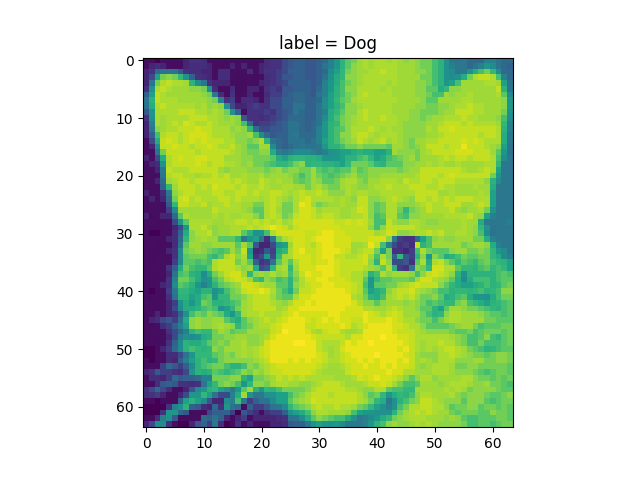
\includegraphics[width=1\linewidth]{2a/pic.png}  
  
  \label{fig:sub-first}
\end{subfigure}
\begin{subfigure}{.5\textwidth}
  \centering
  % include second image
  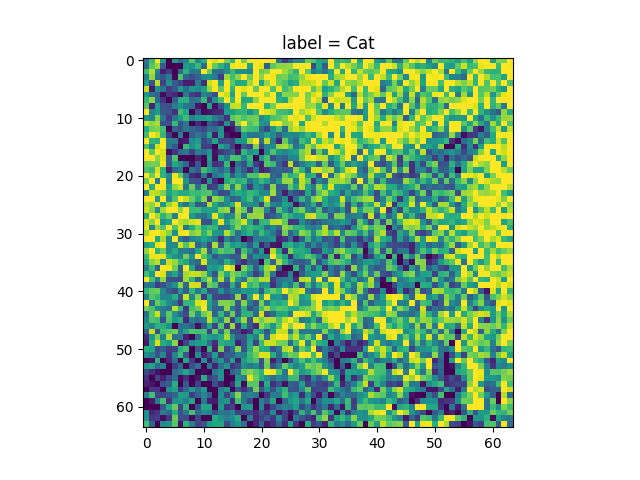
\includegraphics[width=1\linewidth]{2a/Noisy pic.png}  
  
  \label{fig:sub-second}
\end{subfigure}
\caption{Put your caption here}
\label{noise pics}
\end{figure}
\newpage
\section{b}
\subsection{Results}
For this task the first thing which was made was to split every data point (picture) in to 256 features representing 16x16 picture blocks instead of 4096 features. After this the same three models as in the previous task (a) was ran in the exact same manner as before with the only difference being that instead of noise the data was reduced to the 256 features. Since the original picture is made up of 64x64 pixels we get 16 16x16 boxes see figure \ref{BOXES} which we need to get the accuracy for. For each box the procedure was as previous classification exercises ran 100 times and averaged over, the result for the models and standard deviation can be seen in figure \ref{result 2b}. We can see that box 3 (not for logistic regression) and box 5 yield good accuracy and box 8 very poor performance. What box yields good results should be strongly correlated with important features for the classes since if many important features are located in the box the model should preform well hence we can compare with the results in 1b for Random Forest and the logistic regression (Not SVM different kernel used in 1b!). Doing this we would expect almost all boxes to work well for the logistic regression since it had important features spread over the entire picture and for the Random Forest it should only work well for the box around the forhead area. This is however not what we see which is surprising, what we see is that the models seem to follow eachother roughly in which boxes gives good accuracy. Looking at box 3 top left corner fig \ref{BOXES} and box 5 top right corner \ref{BOXES} the first box makes sense since its around the ear which one can imagine differs a lot between the dogs and cats. Box 5  is surprising however since looking at it with the human eye its difficult to make anything out, one explanation could be that pixels in this area generally differ by a lot between cats and dogs. As for Box 8 which is in bottom left corner in fig \ref{BOXES}, which gives poor accuracy scores this area likely has very little information about weather its a cat or not.     
\subsection{Conclusion}
In conclusion one can achieve good accuracy by only looking at a part of the picture it's however not completely straightforward to know which parts yield good results, for example picking an area with important features doesn't seem to be optimal. Furthermore the SVM method once again preformed the best when looking at the optimal Box for this model.
\begin{figure}[H]
    \centering
    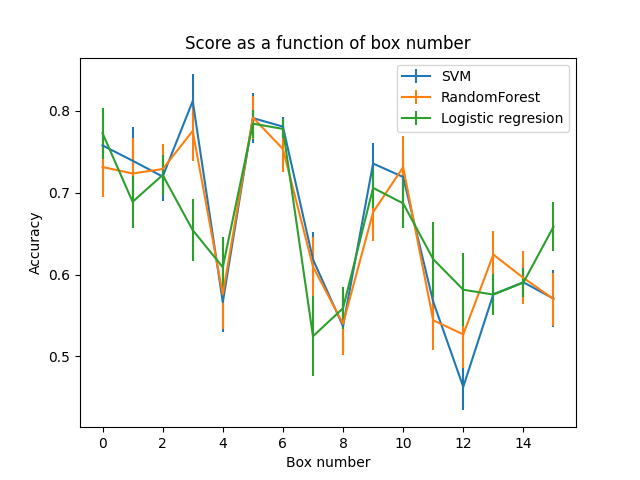
\includegraphics[scale=0.6]{2b/Result.png}
    \caption{Caption}
    \label{result 2b}
\end{figure}
\begin{figure}[H]
\begin{subfigure}{.5\textwidth}
  \centering
  % include first image
  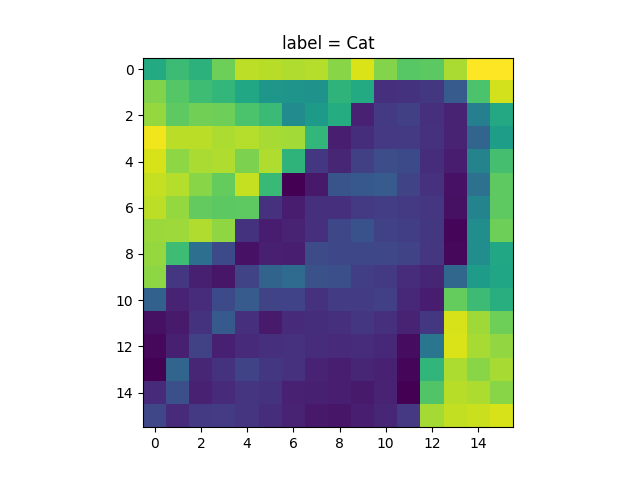
\includegraphics[width=1\linewidth]{2b/Box num 3.png}  
  
  \label{fig:sub-first}
\end{subfigure}
\begin{subfigure}{.5\textwidth}
  \centering
  % include second image
  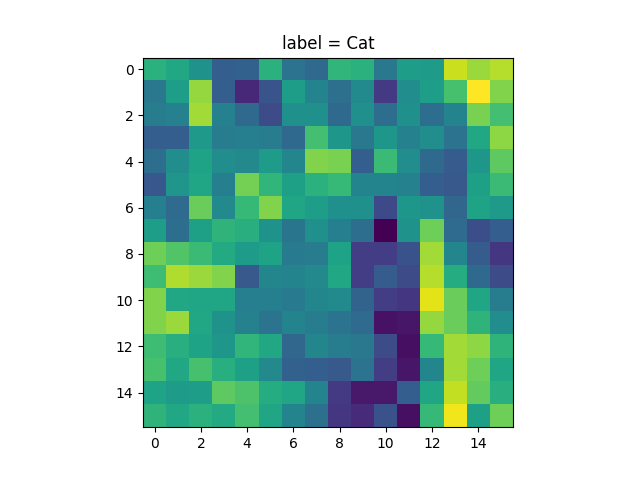
\includegraphics[width=1\linewidth]{2b/box num 5.png}  
  
  \label{fig:sub-second}
\end{subfigure}

\begin{subfigure}{.5\textwidth}
  \centering
  % include first image
  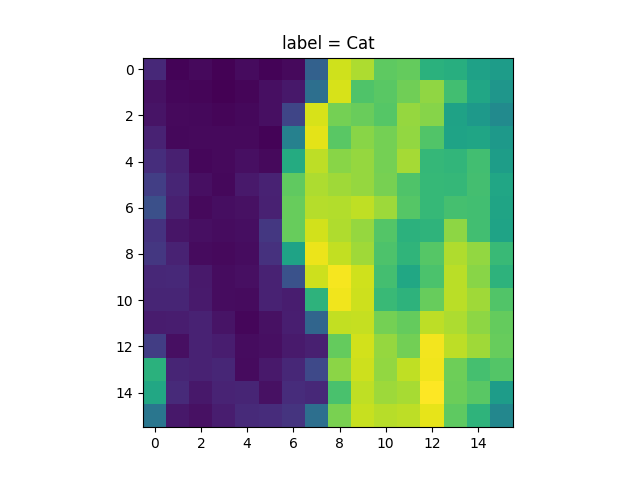
\includegraphics[width=1\linewidth]{2b/box num 8.png}  
  
  \label{fig:sub-first}
\end{subfigure}
\begin{subfigure}{.5\textwidth}
  \centering
  % include first image
  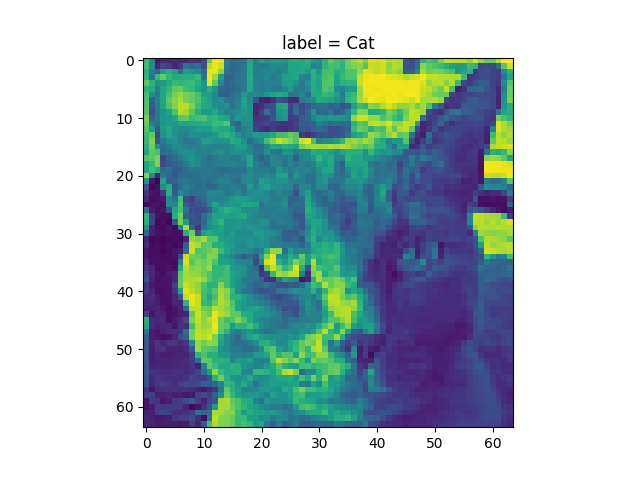
\includegraphics[width=1\linewidth]{2b/example pic.png}  
  
  \label{fig:sub-first}
\end{subfigure}

\caption{Put your caption here}
\label{BOXES}
\end{figure}

\newpage
\section{c}
\subsection{Results}
The same procedure as in 1a and 1b was ran but with half the pictures turned upside down. As for the selected features they are different from 1b for all the models see figure \ref{feet pics} and figure \ref{imp pixels}. There is also a very noticeable effect in performance across all models see table \ref{Rot accuracy} where all the models only preform slightly better than learning nothing at all which would give an score of 0.5. We can also see from the table that the rotated pictures only are slightly over represented in the miss classified pictures which would indicate that the models have an equally hard time classifying upside down images as regular one which is to be expected since half the pictures in the training and test are upside down.    
\subsection{Conclusion}
Rotating the pictures impacts performance greatly and affects feature selection for all models. One can see that many of the previously deemed important features now are completely discarded. The reason for the poor performance could be due to the model not being able to learn the differences between the cats and dogs since the data set is too small for it to be able to learn the difference between upside down dogs and cats in relation to as well learning the difference between the non rotated pictures. The upside down pictures seem to be miss leading the models into not looking for all the important features as in 1b plus some extra for classifying upside down images. Rather the models seem to be looking at some mix of the important features for upside down and regular pictures which gives poor performance. This could perhaps be less of a problem with a bigger sample size as previously stated so an suggestion for performance improvement could be to create your own data from the samples you have.  
\begin{figure}[H]
\begin{subfigure}{.33\textwidth}
  \centering
  % include first image
  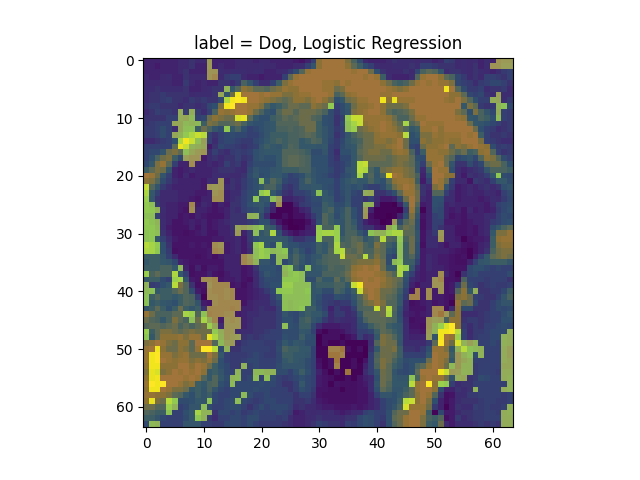
\includegraphics[width=1\linewidth]{2c/Imp feat LR.png}  
  
  \label{fig:sub-first}
\end{subfigure}
\begin{subfigure}{.33\textwidth}
  \centering
  % include second image
  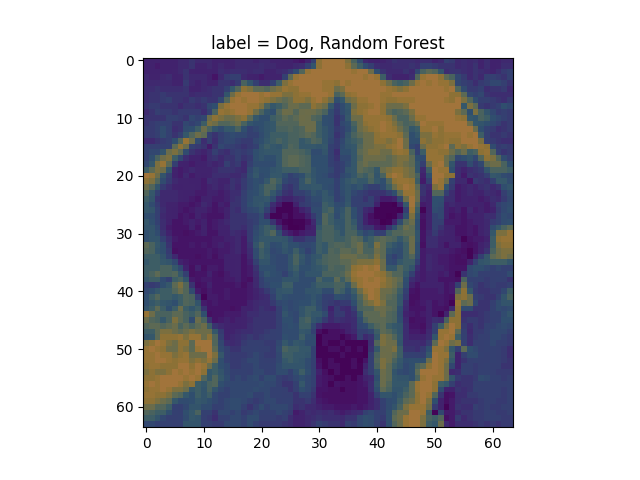
\includegraphics[width=1\linewidth]{2c/Imp feat RF.png}  
  
  \label{fig:sub-second}
\end{subfigure}
\begin{subfigure}{.33\textwidth}
  \centering
  % include second image
  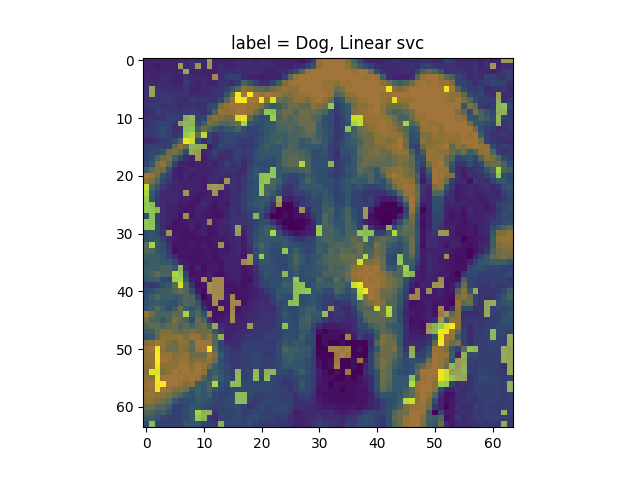
\includegraphics[width=1\linewidth]{2c/Imp feat SVM.png}  
  
  \label{fig:sub-second}
\end{subfigure}
\caption{Put your caption here}
\label{feet pics}
\end{figure}
\begin{figure}[H]
\begin{subfigure}{.33\textwidth}
  \centering
  % include first image
  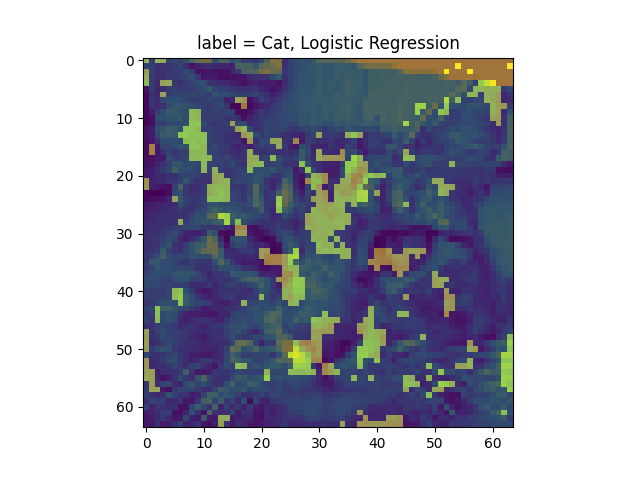
\includegraphics[width=1\linewidth]{1b/Imp_feat LogReg.png}  
  
  \label{RandF}
\end{subfigure}
\begin{subfigure}{.33\textwidth}
  \centering
  % include second image
  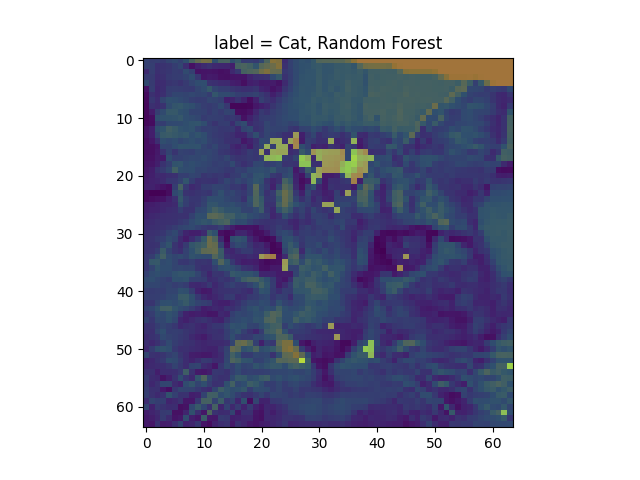
\includegraphics[width=1\linewidth]{1b/Imp_feat RandForest.png}  
  
  \label{fig:sub-second}
\end{subfigure}
\begin{subfigure}{.33\textwidth}
  \centering
  % include second image
  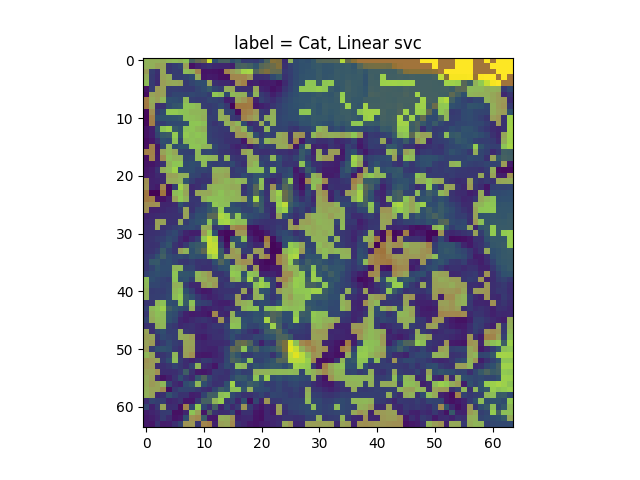
\includegraphics[width=1\linewidth]{1b/Imp_feat_svc.png}  
  
  \label{fig:sub-second}
\end{subfigure}
\caption{Put your caption here}
\label{imp pixels}
\end{figure}
\begin{figure}[H]
\begin{subfigure}{.33\textwidth}
  \centering
  % include first image
  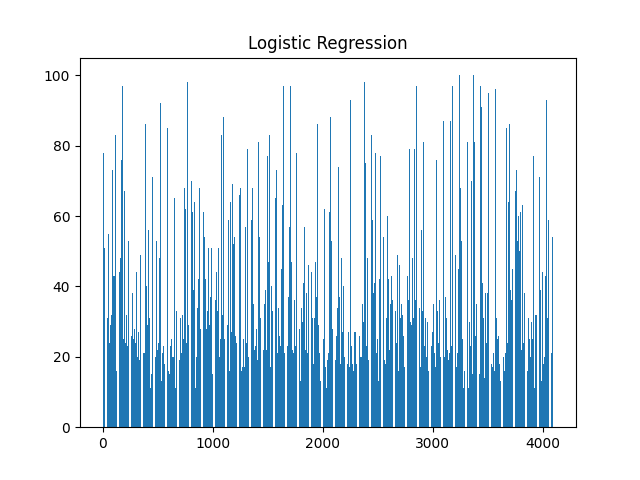
\includegraphics[width=1\linewidth]{2c/Selection LR.png}  
  
  \label{fig:sub-first}
\end{subfigure}
\begin{subfigure}{.33\textwidth}
  \centering
  % include second image
  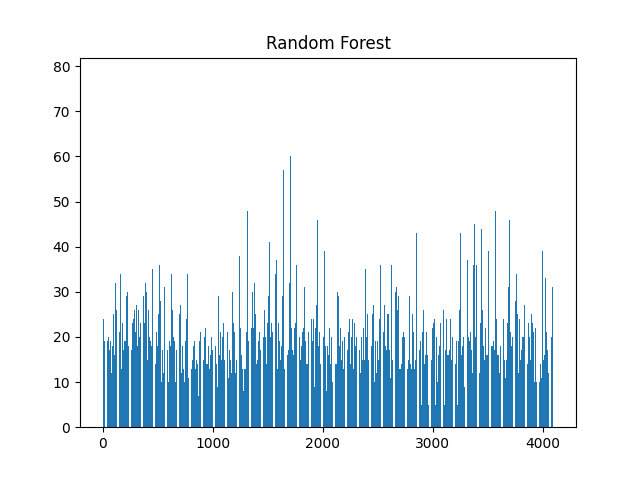
\includegraphics[width=1\linewidth]{2c/Selection RF.png}  
  
  \label{fig:sub-second}
\end{subfigure}
\begin{subfigure}{.33\textwidth}
  \centering
  % include second image
  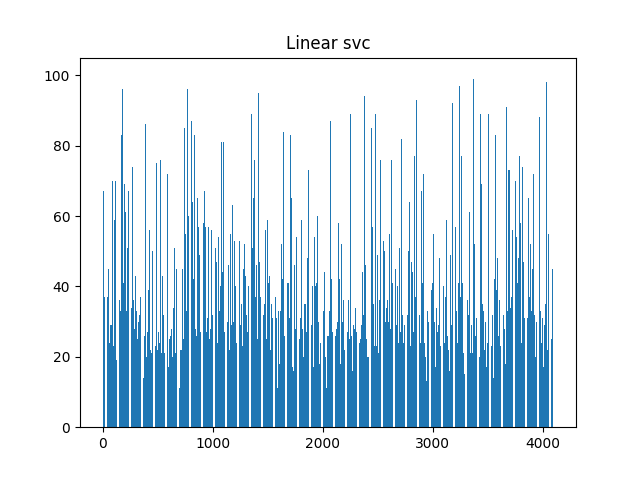
\includegraphics[width=1\linewidth]{2c/Selection SVM.png}  
  
  \label{fig:sub-second}
\end{subfigure}
\caption{Put your caption here}
\label{feet select}
\end{figure}

\begin{table}[H]
    \centering
    \begin{tabular}{c|c|c|c|c|c|c}
         & Accuracy & std & Percentage rotated in miss classified  \\
        SVM & 0.64 & 0.04 & 0.6\\
        Random Forest & 0.65 & 0.07& 0.45\\
        Logistic Regression & 0.64 & 0.06 & 0.54
    \end{tabular}
    \caption{Caption}
    \label{Rot accuracy}
\end{table}
\newpage
\section{d}
\subsection{Results}
For this task only the SVM classifier was looked due to lengthy simulation times, the SVM was chosen since it had the highest accuracy score on the unmodified data set and was therefore deemed as the best. During theese simulation different amount of pixels were modified by changing them to a random value drawn from a uniform distribution U[0, 256] where 5 different levels of pixels were used see table \ref{pixel accuracy}. The results for the accuracy was averaged over 100 runs for each number of pixels and the feature selection was ran with 100 bootstraps for each pixel number.    
\subsection{Conclusion}
\begin{table}[H]
    \centering
    \begin{tabular}{c|c|c|c|c|c|c}
        Number of pixels & 10 &  400  & 1000 & 1500 &2000  \\
        Accuracy & 0.77 & 0.75 & 0.74 & 0.74 & 0.72\\
        std & 0.03 & 0.02& 0.02 & 0.02 & 0.02\\
        
    \end{tabular}
    \caption{Caption}
    \label{pixel accuracy}
\end{table}
\begin{figure}[H]
\begin{subfigure}{.33\textwidth}
  \centering
  % include first image
  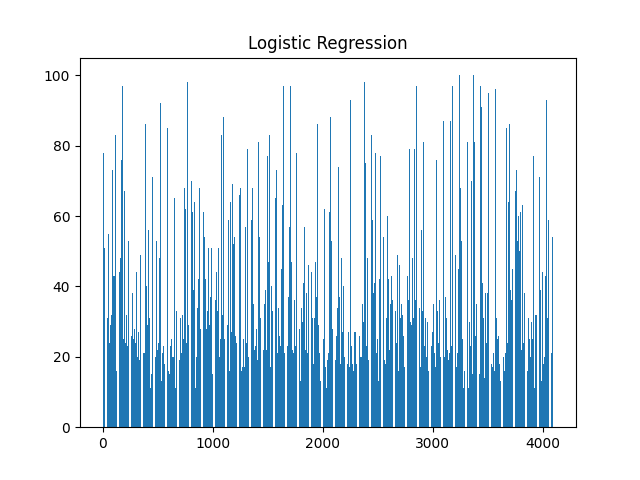
\includegraphics[width=1\linewidth]{2c/Selection LR.png}  
  
  \label{fig:sub-first}
\end{subfigure}
\begin{subfigure}{.33\textwidth}
  \centering
  % include second image
  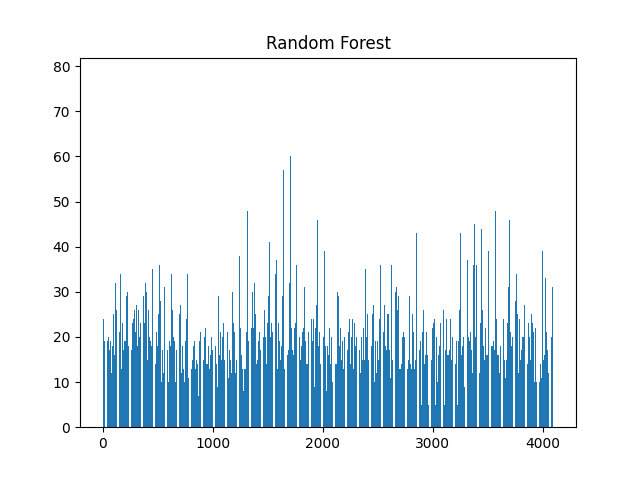
\includegraphics[width=1\linewidth]{2c/Selection RF.png}  
  
  \label{fig:sub-second}
\end{subfigure}
\begin{subfigure}{.33\textwidth}
  \centering
  % include second image
  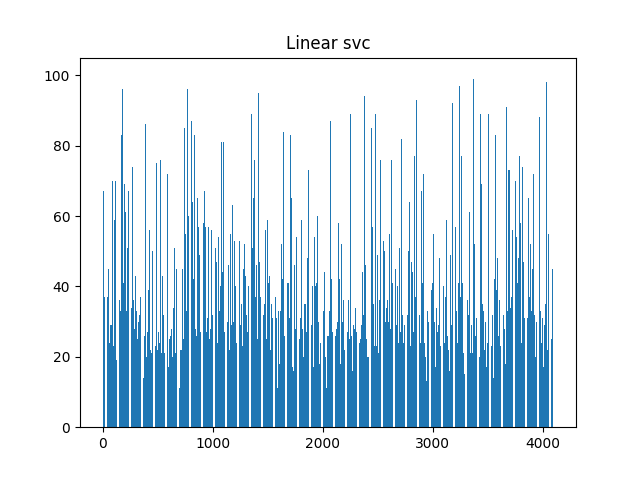
\includegraphics[width=1\linewidth]{2c/Selection SVM.png}  
  
  \label{fig:sub-second}
\end{subfigure}
\caption{Put your caption here}
\label{feet select}
\end{figure}
\newpage
\section{e}
\subsection{Results}
\subsection{Conclusion}
\newpage
\section{f}
\subsection{Results}
\subsection{Conclusion}
\end{document}